\documentclass[10pt]{article}

\usepackage{tabularx}
\usepackage[a4paper,margin=2.5cm, bottom=2.5cm]{geometry}
\usepackage{fancyhdr}
\usepackage{listings}
\usepackage{booktabs}
\usepackage{float}
\usepackage{subcaption}
% \usepackage{caption}
% \captionsetup{font=footnotesize}
\usepackage{graphicx}
\usepackage{amsmath}
\usepackage{amssymb}
\usepackage{amsthm}
\usepackage{array}
\usepackage[table]{xcolor}
\usepackage{pgfplots}
\pgfplotsset{compat=1.17}
\usepackage{pgfplotstable}
\usepackage{multirow}
\usepackage{tikz}
\usepackage[hidelinks]{hyperref}
\usepackage{titling}
\usepackage[polish]{babel} % Polish language support

\setlength{\headheight}{40pt}
\setlength{\parindent}{0pt}
\setlength{\parskip}{1ex}
\renewcommand{\headrulewidth}{0pt}

\pagestyle{fancy}
\fancyhead{}
\fancyhead[L]{
    \renewcommand{\arraystretch}{1.5}
    \begin{tabularx}{\textwidth}{|X|X|}
        \hline
        \bfseries Obliczenia inteligentne & \bfseries \thetitle \\
        \hline
    \end{tabularx}
}
\fancyfoot[C]{\thepage}

\renewcommand{\maketitle}{
    \thispagestyle{plain}
    \renewcommand{\arraystretch}{2}
    \vspace*{-8em}
    \footnotesize
    \begin{flushleft}
        \begin{tabularx}{\textwidth}{|X|X|}
            \hline
            \bfseries Obliczenia Inteligentne  & \bfseries \thetitle                           \\ \hline
            \multicolumn{2}{|l|}{
                \begin{tabular}[t]{@{}ll@{}} 
                    \textbf{Grupa:} Grupa 1
                    \hspace{4.5em}
                    \textbf{Dzień i czas:} Czwartek, 10:00
                    \hspace{4.5em}
                    \textbf{Rok akademicki:} 2023/24
                \end{tabular}
            } \\ \hline
            \multicolumn{2}{|l|}{
                \begin{tabular}[t]{@{}l@{\hspace{10em}}l@{}} 
                    \textbf{Imię i nazwisko:} \textsc{Jakub Pawlak} & \textbf{Imię i nazwisko:} \textsc{Magdalena Paku\l a} 
                \end{tabular}
            } \\
            \hline
        \end{tabularx}
    \end{flushleft}
    \renewcommand{\arraystretch}{1}
}


\title{Projekt 2 --- Zadanie 2}

\captionsetup{font=small}

\newcommand{\plotAccuraciesFromLoggedMetrics}[1]{
    \begin{tikzpicture}
        \begin{axis}[
            width=\linewidth,
            height=.5\linewidth,
            legend pos = south east,
            grid = major,
            style = {font=\small}
        ]
            \addplot+[mark=none] table[x = epoch, y = train_acc] {#1};
            \addlegendentry{Training set accuracy};

            \addplot+[mark=none, orange] table[x = epoch, y = val_acc] {#1};
            \addlegendentry{Test set accuracy};
        \end{axis}
    \end{tikzpicture}
}


\begin{document}

\maketitle
\normalsize

\section{Eksperyment 1: Architektury sieci splotowej dla MNIST (Jakub Pawlak)}\label{sec:ex1-pawlak_mnist}

\subsection*{Pierwsza architektura}


\pgfplotstableread[col sep=comma]{data/kuba/mnist/large.csv}\kubaMnistLarge{}

\begin{figure}[H]\centering
    \begin{subfigure}[t]{.6\textwidth}
        \plotAccuraciesFromLoggedMetrics{\kubaMnistLarge}
        \caption{Wykres zmian accuracy}
    \end{subfigure}
    \hspace{2em}
    \begin{subfigure}[t]{.34\textwidth}
        \centering
        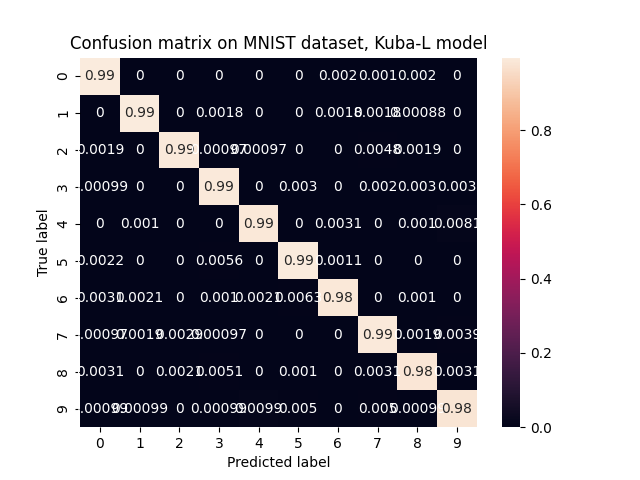
\includegraphics[width=\linewidth]{img/kuba/mnist/large_cm.png}
        \caption{Macierz pomyłek}
    \end{subfigure}
    \caption{Wyniki dla 1 architektury}
\end{figure}


\subsection*{Druga architektura, prowadząca do ekstrakcji 2 cech}

\tiny
\begin{verbatim}
(feature_extractor): Sequential(
    (0): Conv2d(1, 6, kernel_size=(5, 5), stride=(1, 1), padding=(2, 2))
    (1): Sigmoid()
    (2): Dropout2d(p=0.1, inplace=False)
    (3): MaxPool2d(kernel_size=2, stride=2, padding=0, dilation=1, ceil_mode=False)
    (4): Conv2d(6, 16, kernel_size=(5, 5), stride=(1, 1))
    (5): Sigmoid()
    (6): Dropout2d(p=0.1, inplace=False)
    (7): MaxPool2d(kernel_size=2, stride=2, padding=0, dilation=1, ceil_mode=False)
    (8): Conv2d(16, 2, kernel_size=(5, 5), stride=(1, 1))
    (9): Sigmoid()
    (10): Flatten(start_dim=1, end_dim=-1)
)
(classifier): Sequential(
    (0): Linear(in_features=2, out_features=5, bias=True)
    (1): ReLU()
    (2): Linear(in_features=5, out_features=10, bias=True)
)
\end{verbatim}
\normalsize

\pgfplotstableread[col sep=comma]{data/kuba/mnist/smol.csv}\kubaMnistSmol{}

\begin{figure}[H]\centering
    \begin{subfigure}[t]{.6\textwidth}
        \plotAccuraciesFromLoggedMetrics{\kubaMnistSmol}
        \caption{Wykres zmian accuracy}
    \end{subfigure}
    \hspace{2em}
    \begin{subfigure}[t]{.34\textwidth}
        \centering
        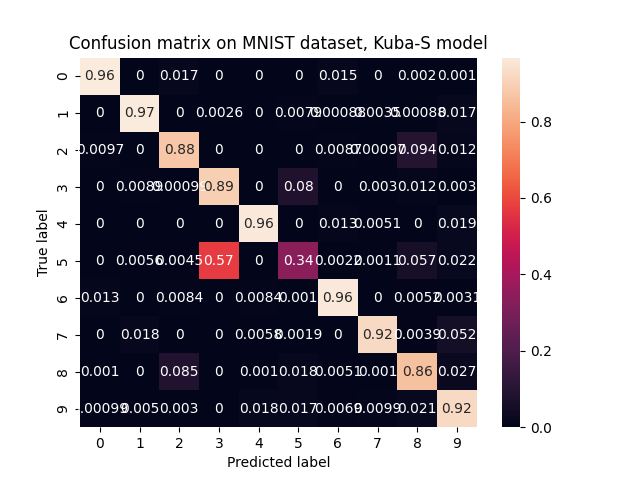
\includegraphics[width=\linewidth]{img/kuba/mnist/smol_cm.png}
        \caption{Macierz pomyłek}
    \end{subfigure}
    \caption{Wyniki dla 2 architektury}
\end{figure}

\pagebreak
\section{Eksperyment 1: Architektury sieci splotowej dla MNIST (Magdalena Pakuła)}\label{sec:ex1-pakula_mnist}

\subsection*{Pierwsza architektura}
Pierwsza architektura sieci składa się z trzech warstw splotowych, po każdej następuje warstwa aktywacji ReLU i warstwy maksymalnego łączenia, a także w pełni połączona warstwa do klasyfikacji.
Wybór trzech warstw splotowych zapewnia równowagę pomiędzy wystarczającą głębokością do uchwycenia złożonych cech a uniknięciem nadmiernej złożoności, która może prowadzić do nadmiernego dopasowania lub wysokich kosztów obliczeniowych.
Po każdej warstwie splotowej następuje aktywacja ReLU i warstwa maksymalnego łączenia. ReLU pomaga we wprowadzeniu nieliniowości, niezbędnej do uczenia się złożonych wzorców, podczas gdy max-pooling zmniejsza wymiary przestrzenne, zmniejszając w ten sposób obciążenie obliczeniowe i pomagając w wyodrębnieniu dominujących cech.
Zastosowanie jąder 5x5 z wypełnieniem w pierwszych dwóch warstwach zapewnia zachowanie wymiarów przestrzennych, umożliwiając sieci nauczenie się lepszych hierarchii przestrzennych w obrazach wejściowych.
Architektura ta osiąga dokładność 98,96\% w przypadku danych testowych przy minimalnej stracie testowej wynoszącej 0,0337 (dla najlepszego modelu, tzn. w 5 epoch).

\begin{figure}[htbp]
    \centering
    \begin{subfigure}[b]{0.2\textwidth}
        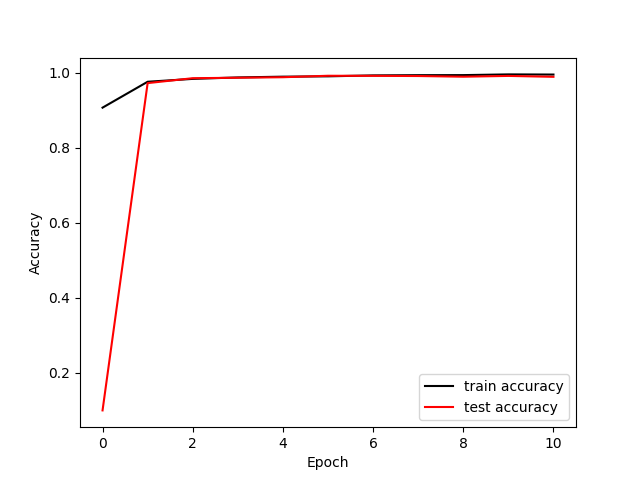
\includegraphics[width=\textwidth]{img/magda/magda_MNIST_1_accuracy_10epochs}
        \caption{Wykres zmian accuracy dla zbioru treningowego i testowego}
        \label{fig:sub1}
    \end{subfigure}
    \begin{subfigure}[b]{0.2\textwidth}
        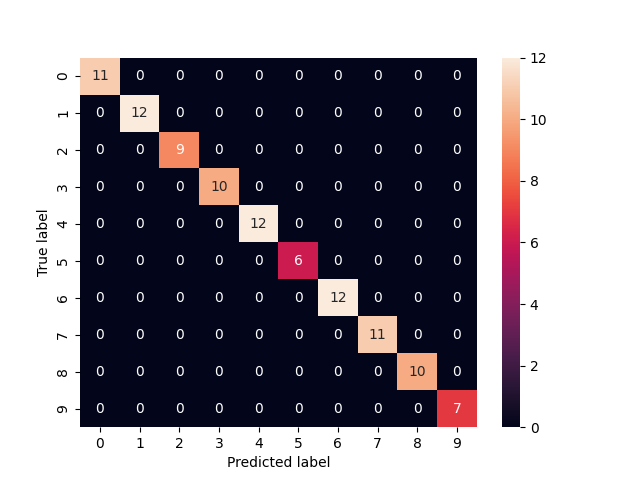
\includegraphics[width=\textwidth]{img/magda/magda_MNIST_1_matrix_best}
        \caption{Macierz pomyłek dla najlepszego modelu}
        \label{fig:sub2}
    \end{subfigure}
    \caption{Wyniki dla 1 architektury}
    \label{fig:eksperyment1_mnist_magda}
\end{figure}

\subsection*{Druga architektura, prowadząca do ekstrakcji 2 cech}
Druga architektura to bardziej kompaktowy CNN zaprojektowany w celu zmniejszenia wymiarowości do 2 cech przed klasyfikacją. Ten prostszy model ma na celu sprawdzenie, jak dobrze może działać wysoce skompresowana reprezentacja. W tym przypadku zostały zastosowane.
Architektura rozpoczyna się od dwóch warstw splotowych, w których zastosowano mniej filtrów (16 i 8) w porównaniu do pierwszego modelu. Ta redukcja ma na celu zmusić sieć do wyodrębnienia najważniejszych informacji.
W warstwie w pełni połączonej elementy (392) są skompresowane do dwóch, co testuje zdolność sieci do destylacji informacji w minimalną reprezentację. Następnie te dwie cechy są odwzorowywane na dziesięć wyników klas, przy czym warstwa aktywacyjna ReLU pomaga zachować nieliniowość w procesie transformacji cech.
Architektura osiąga dokładność danych testowych wynoszącą 81,07\%, przy stracie testowej wynoszącej 0,7146 (dla najlepszego modelu, tzn. w 5 epoch), oferuje ona wgląd w skuteczność redukcji wymiarowości.

\begin{figure}[htbp]
    \centering
    \begin{subfigure}[b]{0.2\textwidth}
        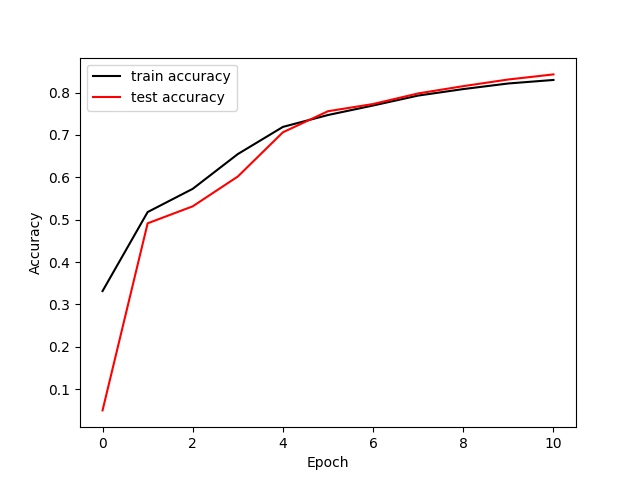
\includegraphics[width=\textwidth]{img/magda/magda_MNIST_2_accuracy_10epochs}
        \caption{Wykres zmian accuracy dla zbioru treningowego i testowego}
        \label{fig:sub3}
    \end{subfigure}
    \begin{subfigure}[b]{0.2\textwidth}
        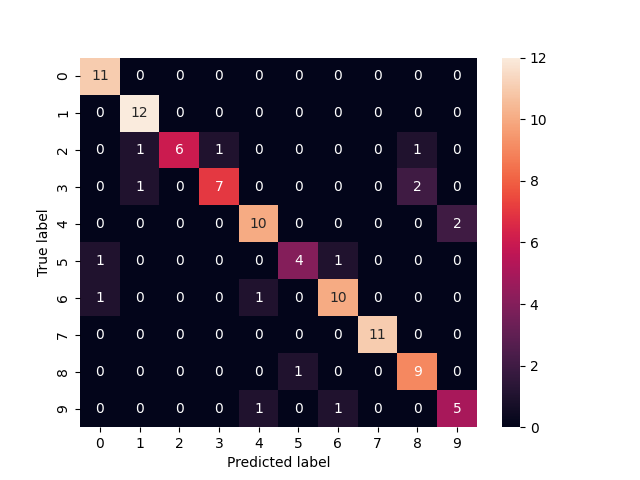
\includegraphics[width=\textwidth]{img/magda/magda_MNIST_2_matrix_best}
        \caption{Macierz pomyłek dla najlepszego modelu}
        \label{fig:sub4}
    \end{subfigure}
    \caption{Wyniki dla 2 architektury}
    \label{fig:eksperyment1_mnist_2_magda}
\end{figure}

\pagebreak
\section{Eksperyment 1: Architektury sieci splotowej dla CIFAR10 (Jakub Pawlak)}\label{sec:ex1-pawlak_cifar}

\paragraph{Pierwsza architektura}
\paragraph{Druga architektura prowadząca do ekstrakcji 2 cech}

\pagebreak
\section{Eksperyment 1: Architektury sieci splotowej dla CIFAR10 (Magdalena Pakuła)}\label{sec:ex1-pakula_cifar}

\paragraph{Pierwsza architektura}
W przypadku tej architektury zostały wybrane dwie warstwy splotowe, po których następują warstwy maksymalnego łączenia w celu zmniejszenia próbkowania map obiektów.
Pierwsza warstwa splotowa posiada 16 filtrów o wymiarach 3x3.
Druga warstwa splotowa posiada 32 filtry o wymiarach 3x3.
Funkcje aktywacji ReLU są stosowane po każdej warstwie splotowej.
Po warstwach splotowych następuje warstwa w pełni połączona z 64 neuronami, po której następuje końcowa warstwa w pełni połączona do klasyfikacji z liczbą neuronów równą liczbie klas (10 dla CIFAR-10).
Wybór takiej architektury pozwala na uchwycenie na obrazach zarówno cech niskiego, jak i wysokiego poziomu. Głębsze warstwy mogą uczyć się bardziej złożonych wzorów i reprezentacji.
Funkcje aktywacji ReLU są używane po każdej warstwie splotowej w celu wprowadzenia nieliniowości, umożliwiając sieci poznanie złożonych relacji między cechami w danych.
W pełni połączona warstwa przed końcową warstwą klasyfikacyjną ma mniej neuronów w porównaniu z warstwą poprzednią. To zmniejszenie złożoności pomaga w nauce bardziej zwartej reprezentacji przestrzeni cech, potencjalnie redukując nadmierne dopasowanie i obciążenie obliczeniowe.

\paragraph{Druga architektura prowadząca do ekstrakcji 2 cech}
Druga architektura jest dosyć podobna do pierwszej, tzn. pierwsza wartwa wygląda tak samo, lecz druga warstwa posiada 16 filtrów o wymiarach 3x3.
Po warstwach splotowych następuje warstwa w pełni połączona, zawierająca tylko 2 neurony. Następnie jest końcowa, w pełni połączona warstwa do klasyfikacji z liczbą neuronów równą liczbie klas

\pagebreak
\section{Eksperyment 2: Wyniki dla MNIST}\label{sec:ex2_mnist}

\paragraph{Najlepsza architektura}
\paragraph{Najelpsza architektura prowadząca do ekstrakcji 2 cech}

\pagebreak
\section{Eksperyment 2: Wyniki dla CIFAR10}\label{sec:ex2_cifar}

\paragraph{Najlepsza architektura}
\paragraph{Najelpsza architektura prowadząca do ekstrakcji 2 cech}

\pagebreak
\section{Analiza i wnioski}\label{sec:wyniki}

\paragraph{Porównanie architektur sieci splotowych}

\paragraph{Wpływ augmentacji danych}

\end{document}